\documentclass[12pt,letterpaper]{hmcpset}
\usepackage[margin=1in]{geometry}
\usepackage{graphicx}
\usepackage{amsthm}
\usepackage{enumitem}

% Theorems
\usepackage{amsthm}
\renewcommand\qedsymbol{$\blacksquare$}
\makeatletter
\@ifclassloaded{article}{
    \newtheorem{definition}{Definition}[section]
    \newtheorem{example}{Example}[section]
    \newtheorem{theorem}{Theorem}[section]
    \newtheorem{corollary}{Corollary}[theorem]
    \newtheorem{lemma}{Lemma}[theorem]
}{
}
\makeatother

% Random Stuff
\setlength\unitlength{1mm}

\newcommand{\insertfig}[3]{
\begin{figure}[htbp]\begin{center}\begin{picture}(120,90)
\put(0,-5){\includegraphics[width=12cm,height=9cm,clip=]{#1.eps}}\end{picture}\end{center}
\caption{#2}\label{#3}\end{figure}}

\newcommand{\insertxfig}[4]{
\begin{figure}[htbp]
\begin{center}
\leavevmode \centerline{\resizebox{#4\textwidth}{!}{\input
#1.pstex_t}}
\caption{#2} \label{#3}
\end{center}
\end{figure}}

\long\def\comment#1{}

\newcommand\norm[1]{\left\lVert#1\right\rVert}
\DeclareMathOperator*{\argmin}{arg\,min}
\DeclareMathOperator*{\argmax}{arg\,max}

% bb font symbols
\newfont{\bbb}{msbm10 scaled 700}
\newcommand{\CCC}{\mbox{\bbb C}}

\newfont{\bbf}{msbm10 scaled 1100}
\newcommand{\CC}{\mbox{\bbf C}}
\newcommand{\PP}{\mbox{\bbf P}}
\newcommand{\RR}{\mbox{\bbf R}}
\newcommand{\QQ}{\mbox{\bbf Q}}
\newcommand{\ZZ}{\mbox{\bbf Z}}
\renewcommand{\SS}{\mbox{\bbf S}}
\newcommand{\FF}{\mbox{\bbf F}}
\newcommand{\GG}{\mbox{\bbf G}}
\newcommand{\EE}{\mbox{\bbf E}}
\newcommand{\NN}{\mbox{\bbf N}}
\newcommand{\KK}{\mbox{\bbf K}}
\newcommand{\KL}{\mbox{\bbf KL}}

% Vectors
\renewcommand{\aa}{{\bf a}}
\newcommand{\bb}{{\bf b}}
\newcommand{\cc}{{\bf c}}
\newcommand{\dd}{{\bf d}}
\newcommand{\ee}{{\bf e}}
\newcommand{\ff}{{\bf f}}
\renewcommand{\gg}{{\bf g}}
\newcommand{\hh}{{\bf h}}
\newcommand{\ii}{{\bf i}}
\newcommand{\jj}{{\bf j}}
\newcommand{\kk}{{\bf k}}
\renewcommand{\ll}{{\bf l}}
\newcommand{\mm}{{\bf m}}
\newcommand{\nn}{{\bf n}}
\newcommand{\oo}{{\bf o}}
\newcommand{\pp}{{\bf p}}
\newcommand{\qq}{{\bf q}}
\newcommand{\rr}{{\bf r}}
\renewcommand{\ss}{{\bf s}}
\renewcommand{\tt}{{\bf t}}
\newcommand{\uu}{{\bf u}}
\newcommand{\ww}{{\bf w}}
\newcommand{\vv}{{\bf v}}
\newcommand{\xx}{{\bf x}}
\newcommand{\yy}{{\bf y}}
\newcommand{\zz}{{\bf z}}
\newcommand{\0}{{\bf 0}}
\newcommand{\1}{{\bf 1}}

% Matrices
\newcommand{\Ab}{{\bf A}}
\newcommand{\Bb}{{\bf B}}
\newcommand{\Cb}{{\bf C}}
\newcommand{\Db}{{\bf D}}
\newcommand{\Eb}{{\bf E}}
\newcommand{\Fb}{{\bf F}}
\newcommand{\Gb}{{\bf G}}
\newcommand{\Hb}{{\bf H}}
\newcommand{\Ib}{{\bf I}}
\newcommand{\Jb}{{\bf J}}
\newcommand{\Kb}{{\bf K}}
\newcommand{\Lb}{{\bf L}}
\newcommand{\Mb}{{\bf M}}
\newcommand{\Nb}{{\bf N}}
\newcommand{\Ob}{{\bf O}}
\newcommand{\Pb}{{\bf P}}
\newcommand{\Qb}{{\bf Q}}
\newcommand{\Rb}{{\bf R}}
\newcommand{\Sb}{{\bf S}}
\newcommand{\Tb}{{\bf T}}
\newcommand{\Ub}{{\bf U}}
\newcommand{\Wb}{{\bf W}}
\newcommand{\Vb}{{\bf V}}
\newcommand{\Xb}{{\bf X}}
\newcommand{\Yb}{{\bf Y}}
\newcommand{\Zb}{{\bf Z}}

% Calligraphic
\newcommand{\Ac}{{\cal A}}
\newcommand{\Bc}{{\cal B}}
\newcommand{\Cc}{{\cal C}}
\newcommand{\Dc}{{\cal D}}
\newcommand{\Ec}{{\cal E}}
\newcommand{\Fc}{{\cal F}}
\newcommand{\Gc}{{\cal G}}
\newcommand{\Hc}{{\cal H}}
\newcommand{\Ic}{{\cal I}}
\newcommand{\Jc}{{\cal J}}
\newcommand{\Kc}{{\cal K}}
\newcommand{\Lc}{{\cal L}}
\newcommand{\Mc}{{\cal M}}
\newcommand{\Nc}{{\cal N}}
\newcommand{\Oc}{{\cal O}}
\newcommand{\Pc}{{\cal P}}
\newcommand{\Qc}{{\cal Q}}
\newcommand{\Rc}{{\cal R}}
\newcommand{\Sc}{{\cal S}}
\newcommand{\Tc}{{\cal T}}
\newcommand{\Uc}{{\cal U}}
\newcommand{\Wc}{{\cal W}}
\newcommand{\Vc}{{\cal V}}
\newcommand{\Xc}{{\cal X}}
\newcommand{\Yc}{{\cal Y}}
\newcommand{\Zc}{{\cal Z}}

% Bold greek letters
\newcommand{\alphab}{\hbox{\boldmath$\alpha$}}
\newcommand{\betab}{\hbox{\boldmath$\beta$}}
\newcommand{\gammab}{\hbox{\boldmath$\gamma$}}
\newcommand{\deltab}{\hbox{\boldmath$\delta$}}
\newcommand{\etab}{\hbox{\boldmath$\eta$}}
\newcommand{\lambdab}{\hbox{\boldmath$\lambda$}}
\newcommand{\epsilonb}{\hbox{\boldmath$\epsilon$}}
\newcommand{\nub}{\hbox{\boldmath$\nu$}}
\newcommand{\mub}{\hbox{\boldmath$\mu$}}
\newcommand{\zetab}{\hbox{\boldmath$\zeta$}}
\newcommand{\phib}{\hbox{\boldmath$\phi$}}
\newcommand{\psib}{\hbox{\boldmath$\psi$}}
\newcommand{\thetab}{\hbox{\boldmath$\theta$}}
\newcommand{\taub}{\hbox{\boldmath$\tau$}}
\newcommand{\omegab}{\hbox{\boldmath$\omega$}}
\newcommand{\xib}{\hbox{\boldmath$\xi$}}
\newcommand{\sigmab}{\hbox{\boldmath$\sigma$}}
\newcommand{\pib}{\hbox{\boldmath$\pi$}}
\newcommand{\rhob}{\hbox{\boldmath$\rho$}}

\newcommand{\Gammab}{\hbox{\boldmath$\Gamma$}}
\newcommand{\Lambdab}{\hbox{\boldmath$\Lambda$}}
\newcommand{\Deltab}{\hbox{\boldmath$\Delta$}}
\newcommand{\Sigmab}{\hbox{\boldmath$\Sigma$}}
\newcommand{\Phib}{\hbox{\boldmath$\Phi$}}
\newcommand{\Pib}{\hbox{\boldmath$\Pi$}}
\newcommand{\Psib}{\hbox{\boldmath$\Psi$}}
\newcommand{\Thetab}{\hbox{\boldmath$\Theta$}}
\newcommand{\Omegab}{\hbox{\boldmath$\Omega$}}
\newcommand{\Xib}{\hbox{\boldmath$\Xi$}}

% mixed symbols
\newcommand{\sinc}{{\hbox{sinc}}}
\newcommand{\diag}{{\hbox{diag}}}
\renewcommand{\det}{{\hbox{det}}}
% \newcommand{\trace}{{\hbox{tr}}}
% \newcommand{\tr}{\trace}
\newcommand{\sign}{{\hbox{sign}}}
\renewcommand{\arg}{{\hbox{arg}}}
\newcommand{\var}{{\hbox{var}}}
\newcommand{\cov}{{\hbox{cov}}}
\renewcommand{\Re}{{\rm Re}}
\renewcommand{\Im}{{\rm Im}}
\newcommand{\eqdef}{\stackrel{\Delta}{=}}
\newcommand{\defines}{{\,\,\stackrel{\scriptscriptstyle \bigtriangleup}{=}\,\,}}
\newcommand{\<}{\left\langle}
\renewcommand{\>}{\right\rangle}
\newcommand{\Psf}{{\sf P}}
\newcommand{\T}{\top}
\newcommand{\m}[1]{\begin{bmatrix} #1 \end{bmatrix}}


\usepackage{fourier}
\usepackage{physics}


% info for header block in upper right hand corner
\name{Colin Adams}
\class{Math189R SU20}
\assignment{Homework 1}
\duedate{Monday, June 2020}

\renewcommand{\labelenumi}{{(\alph{enumi})}}


\begin{document}
Feel free to work with other students, but make sure you write up the homework
and code on your own (no copying homework \textit{or} code; no pair programming).
Feel free to ask students or instructors for help debugging code or whatever else,
though.
The starter code for problem 2 part c and d can be found under the Resource tab on course website.\\

\textit{Note:} You need to create a Github account for submission of the coding part of the homework. Please create a repository on Github to hold all your code and include your Github account username as part of the answer to problem 2.

\begin{problem}[Linear Transformation]
Let $\mathbf{y} = A\mathbf{x} + \mathbf{b}$ be a random vector.
Show that expectation is linear:
\[
    \EE[\yy] = \EE[A\xx + \bb] = A\EE[\xx] + \bb.
\]
Also show that
\[
    \cov[\yy] = \cov[A\xx + \bb] = A \cov[\xx] A^\T = A\Sigmab A^\T.
\]
\end{problem}
\begin{solution}
    For the first part, we have 
    \begin{align*}
         \EE[\yy] = \EE[A\xx + \bb] \equiv \int (A \xx  + \bb) p(\xx) \dd{\xx} = A \int \xx \dd{\xx} + \int \bb p(\xx) \dd{\xx}.
    \end{align*}
    Using the definition of $\EE[\xx] \equiv \int \xx \dd{\xx}$ and since $A$ and $\bb$ are independent of $\xx$, and---lastly---because $\int p(\xx) \dd{\xx} = 1$, we have
    \begin{align*}
         \EE[\yy] = \EE[A\xx + \bb] = A\EE[\xx] + \bb
    \end{align*}
    as desired.

    As for the second part, we have a similar strategy. Since the covariance is defined to be  $\cov[\xx] \equiv \EE[(\xx - \EE[\xx])(\xx - \EE[\xx])^T]$, we have
    \begin{align*}
         \cov[\yy] = \cov[A\xx + \bb] &\equiv  \EE[(A\xx + \bb - \EE[A\xx + \bb])(A\xx + \bb - \EE[A\xx + \bb])^T] \\
         &= \EE[(A\xx + \bb - A\EE[\xx]  -\bb)(A\xx + \bb - A\EE[\xx]  -\bb)^T] &\qq{(result from above)} \\
         &=\EE[(A\xx - A\EE[\xx])(A\xx  - A\EE[\xx])^T] \\
         &= \EE[(A(\xx - \EE[\xx]))(A(\xx - \EE[\xx]))^T] \\
         &= A\EE[(\xx - \EE[\xx]))(\xx - \EE[\xx])^T] A^T \\
         &= A \cov[\xx] A^T &\qq{(def.\ of covariance)} \\
         &= A \Sigmab A^T
    \end{align*}
    as desired.
\end{solution}
\newpage




\begin{problem}[2]
Given the dataset $\Dc = \{(x,y)\} = \{(0,1), (2,3), (3,6), (4,8)\}$
\begin{enumerate}
   \item Find the least squares estimate $y = \thetab^\T\xx$ by hand using
        Cramer's Rule.
    \item Use the normal equations to find the same solution and verify it
        is the same as part (a).
    \item Plot the data and the optimal linear fit you found.
    \item Find randomly generate 100 points near the line with white Gaussian
        noise and then compute the least squares estimate (using a computer).
        Verify that this new line is close to the original and plot the new
        dataset, the old line, and the new line.
\end{enumerate}

\end{problem}
\begin{solution}
    This seems like it's going to be a bit tedious.
    \begin{enumerate}
        \item We are hoping to solve for $y = m x + b$ for the least squares estimate using our data. There is a messy formula which I guess we will solve for. Notice the length of $\mathcal D = 4$. Also note the following 
        \begin{align*}
            \sum_i x_i = 9, \qq{} \sum_i x_i^2 = 29, \qq{} \sum_i y_i = 18, \qq{} \sum_i y_i^2 = 110,  \qq{} \sum_i x_iy_i = 56
        \end{align*}
        which we plug into this hideous beasts of 
        \begin{align*}
            m = \frac{n \sum_i x_iy_i - \qty(\sum_i x_i) \qty(\sum_i y_i) }{n \sum_i x_i^2 - \qty(\sum_i x_i)^2}
            \qq{and}
            b = \frac{\qty(\sum_i x_i^2)\qty(\sum_i y_i) - \qty(\sum_i x_i)\qty(\sum_i x_iy_i)}{n \sum_i x_i^2 - \qty(\sum_i x_i)^2}
        \end{align*}
        which we evaluate and get
        \begin{align*}
            m = \frac{62}{35}
            \qq{and}
            b = \frac{18}{35}
        \end{align*}
        which gives us our old friend $y = mx + b$ as a fit for the data.

        \item Now, we use the normal equations to find this solution. We write 
        \begin{align*}
            \vb X = \mqty[1 & 0 \\ 
                         1 & 2 \\
                         1 & 3 \\
                         1 & 4   
                            ], \qq{} \vb y = \mqty[ 1\\ 3\\6\\8], \qq{and} \thetab = \mqty[b \\m].
        \end{align*}
        Using these allows us to evaluate the normal equations
        \begin{align*}
            \thetab &= (\vb X^T \vb X)^{-1}\vb X^T \vb y  = \qty( \mqty[1 & 1 & 1 & 1 \\
 0 & 2 & 3 & 4   
                            ] \mqty[1 & 0 \\ 
                         1 & 2 \\
                         1 & 3 \\
                         1 & 4   
                            ] )^{-1} \mqty[1 & 1 & 1 & 1 \\
 0 & 2 & 3 & 4]
                         \mqty[ 1\\ 3\\6\\8] = \frac{1}{35} \mqty[18 \\ 62 ]
        \end{align*}
        which is the result we expected. 

        \item[(c)\&(d)] Now we will make the plot of our optimal linear fit as well as the one with the random noise.
        \begin{center}
            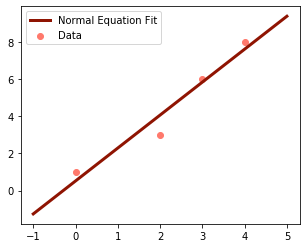
\includegraphics[width = 3in]{data_plot.png} 
            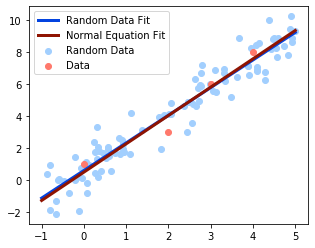
\includegraphics[width = 3.05in]{random_plot.png}
        \end{center}
        These agree quite nicely with one another.
    \end{enumerate}
\end{solution}
\newpage



\end{document}

